% !TEX root = main.tex
\chapter{Decay-time fit}


\section{Fit to data}

% Zeitrange muss hier genannt/beschrieben werden

\subsection{Decay time resolution}
\label{sec:resolution}

Since the work in this section was done by a collaborator, the contents are described for the sake of completeness, but smaller details are omitted.

The decay-time resolution is determined on a sample of \emph{fake} \Bz-candidates, formed from a prompt \Dpm candidate and another track originating from the PV.
The candidates are selected with the same selection as presented in \cref{sec:selection} except for the cut on the BDT output.
Additioanally, the \emph{fake} \Bz-candidates are required to have an impact parameter $\chi^2$ with the PV is less than nine and the number of \ac{PV}s in the event must be one to exclude wrong \ac{PV} associations.
Subsequently \emph{sWeights} are determined by a fit to the invariant mass of the \Dpm meson in order to examine only signal distributions in the following.
Since the time resolution depends on the transverse momentum of the bachelor particle, as a last preparatory step, this need to be corrected in the sample of \emph{fake} \Bz-candidates.
Therefore the prompt sample is weighted by the ratio of the distributions of the logarithmic transverse momenta of the bachelor candidate in the signal \BdToDpi and the prompt sample.

To resolve the decay-time resolution, fits are then performed to the decay-time distribution of the prompt sample in \num{20} bins of the decay-time error.
Since this sample does not contain real \Bz candidates, the decay time is expected to be zero and the decay-time resolution can be derived from the width of the distribution.
The binning is chosen so that the sum of \emph{sWeights} in each bin is equal.
The fit model consists of three components: A delta function convolved with a Gaussian function to describe the true \Dpm+track component, a pair of exponential functions convolved with the same Gaussian function to describe candidates from \bquark-hadron and a wide Gaussian function to describe backgrounds due to wrongly associated \ac{PV}s.
The fit is shown for one representative bin in \cref{fig:resolutionRepresentativeBin}.
\begin{figure}[tbp]
    \centering
    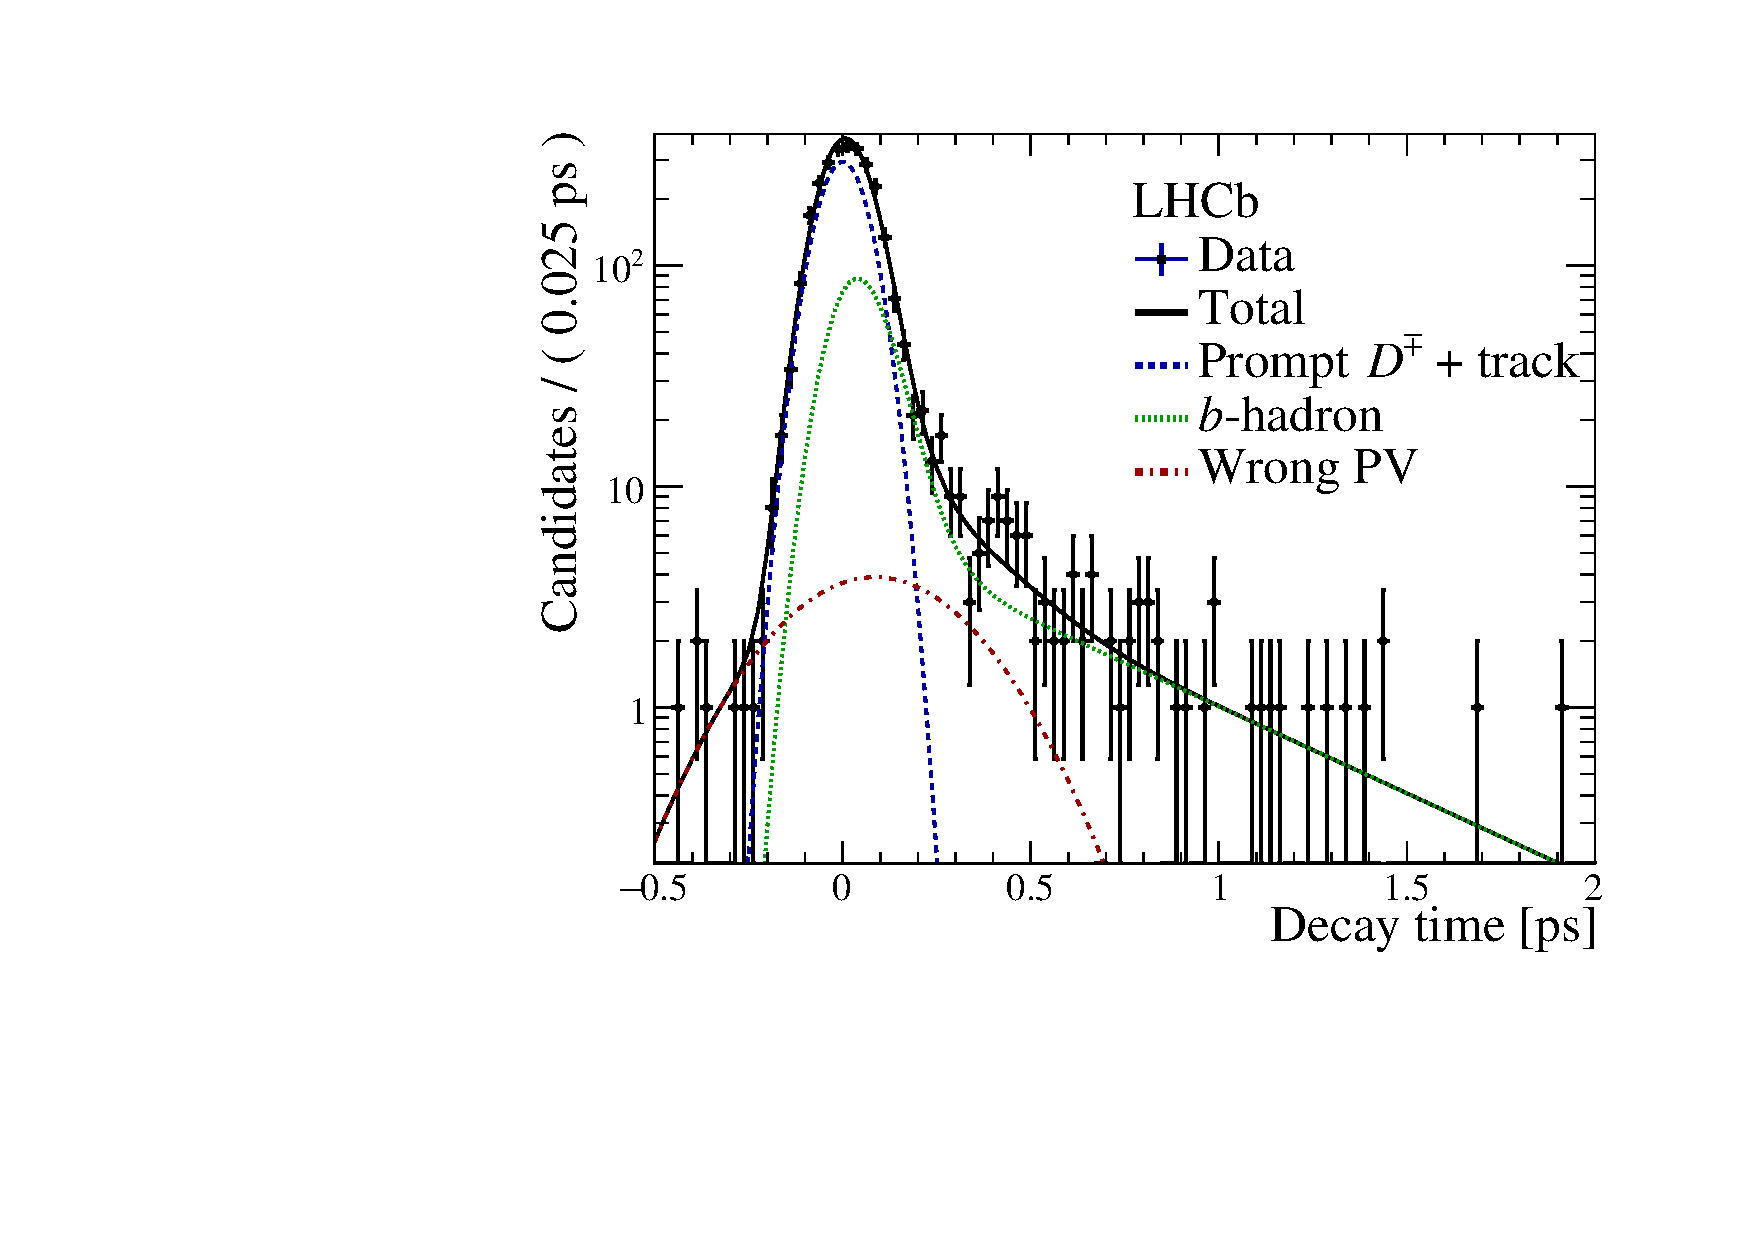
\includegraphics[width=0.48\textwidth]{09TimeFit/figs/resolution_Bin15.pdf}
    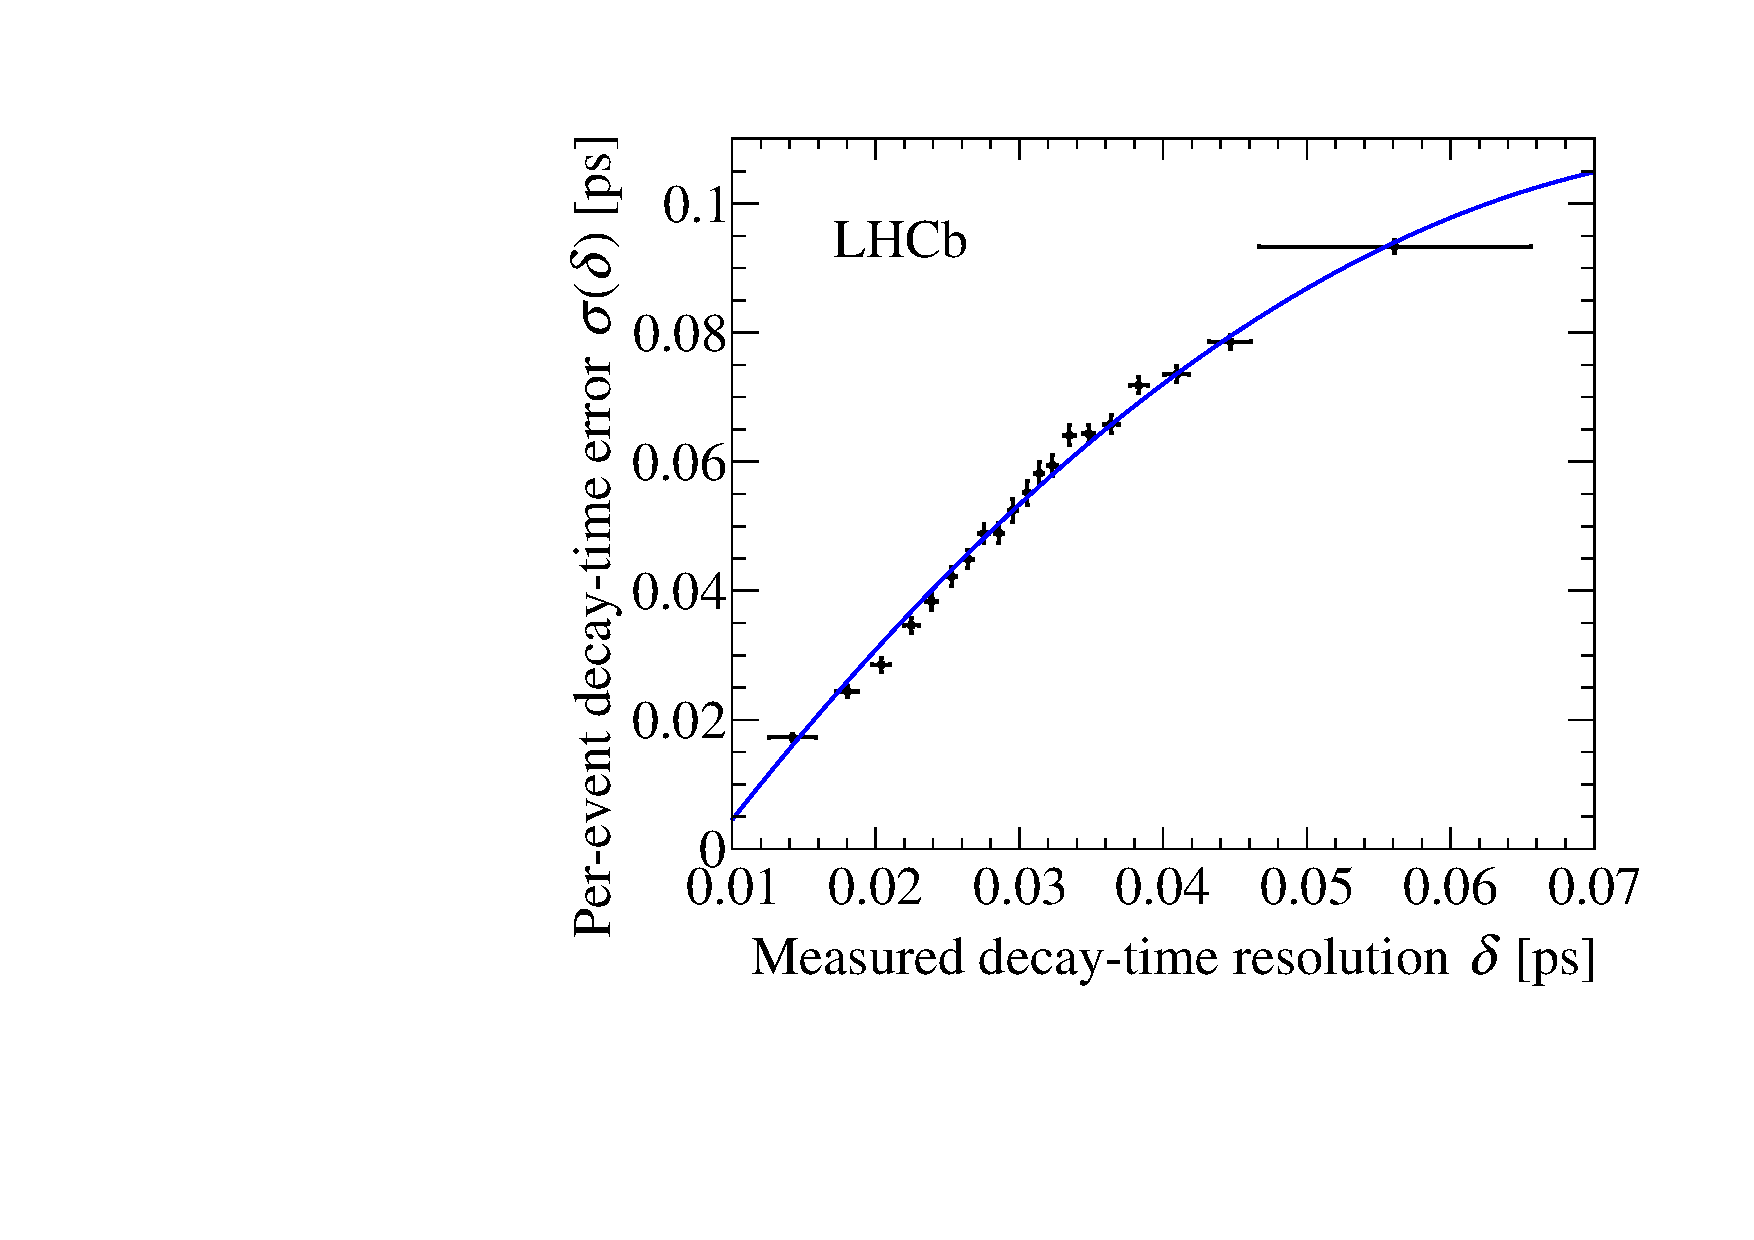
\includegraphics[width=0.48\textwidth]{09TimeFit/figs/resolution_chi2Fit.pdf}
    \caption{Left: Decay-time resolution for one representative bin in per-candidate decay-time error for \emph{fake} \Bz candidates.
    Right: Measured resolution versus average per-candidate decay-time error, determined from fits to the decay time in bins of decay-time error.}
    \label{fig:resolutionRepresentativeBin}
\end{figure}
From this fit a measured resolution $\left<\sigma\right>_i$ per bin is obtained, which can be related to the corresponding average decay-time error $\left<\delta\right>_i$.
Following a $\chi^2$ is fit to the $(\left<\delta\right>_i, \left<\sigma\right>_i)$ pairs of the form
\begin{equation}
\left<\sigma\right>_i=\left<\sigma\right>+p_1\times\left(\left<\delta\right>_i-\left<\delta\right>\right)+p_2\times\left(\left<\delta\right>_i-\left<\delta\right>\right)^2
\end{equation}
is performed, where $\left<\delta\right>$ is the average per-event decay-time error of the whole unbinned sample.
This $\chi^2$ fit, shown in \cref{fig:resolutionRepresentativeBin}, provides an average decay time resolution $\left<\sigma\right>$ and a trend.
From this, a global average resolution of \mbox{$\sigma\!\left(\left<\delta\right>\right)=\SI{0.05491\pm0.00038}{\pico\second}$} can be determined.

\subsection{Decay-time dependent efficiency}
\label{sec:acceptance}

Due to some selection criteria and trigger requirements, as well as inefficiencies in \velo reconstruction, the detector efficiency is not constant over the \Bz decay-time.
This efficiency, hereinafter referred to as acceptance, goes very quickly towards zero for low decay times, reaches a plateau for intermediate decay times, and drops slightly again at high decay times.

For this analysis two models were developed in parallel, which give almost identical results for the \CP parameters \Sf and \Sfbar.
The model used in the final decay-time fit was developed by a collaborator and has one degree of freedom more, while the model described below is used as a crosscheck and for estimating systematic uncertainties.
In both models the acceptance is defined by splines, which are defined analytically in the decay-time fit as described in Ref.~\cite{Karbach:2014qba}.
These splines consist of cubic polynomials defined piecewise in decay-time.
The model is then defined by the limits of the ranges on which the cubic polynomials (also denoted as knots) are defined and associated coefficients, of which two more than knots are required.

The parameterisation described below belongs to the second model developed by myself.
The model is optimised in order to to find the ideal knot  positions giving a good descirption of the decay-time with the minimum number of knots at the same time.
This is done on simulated events by performing a maximum-likelihood fit to the decay-time with the PDF defined as
\begin{equation}
\mathcal{A}(t)\propto a(t)\int dt' \mathcal{R}\!\left(t-t'\right)e^{\,\nicefrac{t'}{\tau}}
\end{equation}
where the resolution $\mathcal{R}\!\left(t-t'\right)$ is taken from \cref{sec:resolution} and the lifetime $\tau$ is fixed to the value used in the generation.
Then it is further checked if the obtained model also describes the \emph{sWeighted} decay-time distribution in the \BdToDpi sample satisfactorily.
Instead of fixing the lifetime, on data it is constraint by means of a Gaussian function to the world average $\tau=\SI{1.518\pm0.004}{\pico\second}$~\cite{PDG_2017}.
A good description was found using seven knots at $[0.4, 0.45, 0.8, 1.3, 2.5, 6.0, 12.0]\,$\si{\pico\second}, where the coefficient at \SI{2.5}{\pico\second} is set to one to fix the overall normalisation.
Figure \ref{fig:acceptance} shows a graphical representation of the used parameterisation with the coefficients obtained on \BdToDpi data.
\begin{figure}[tbp]
    \centering
    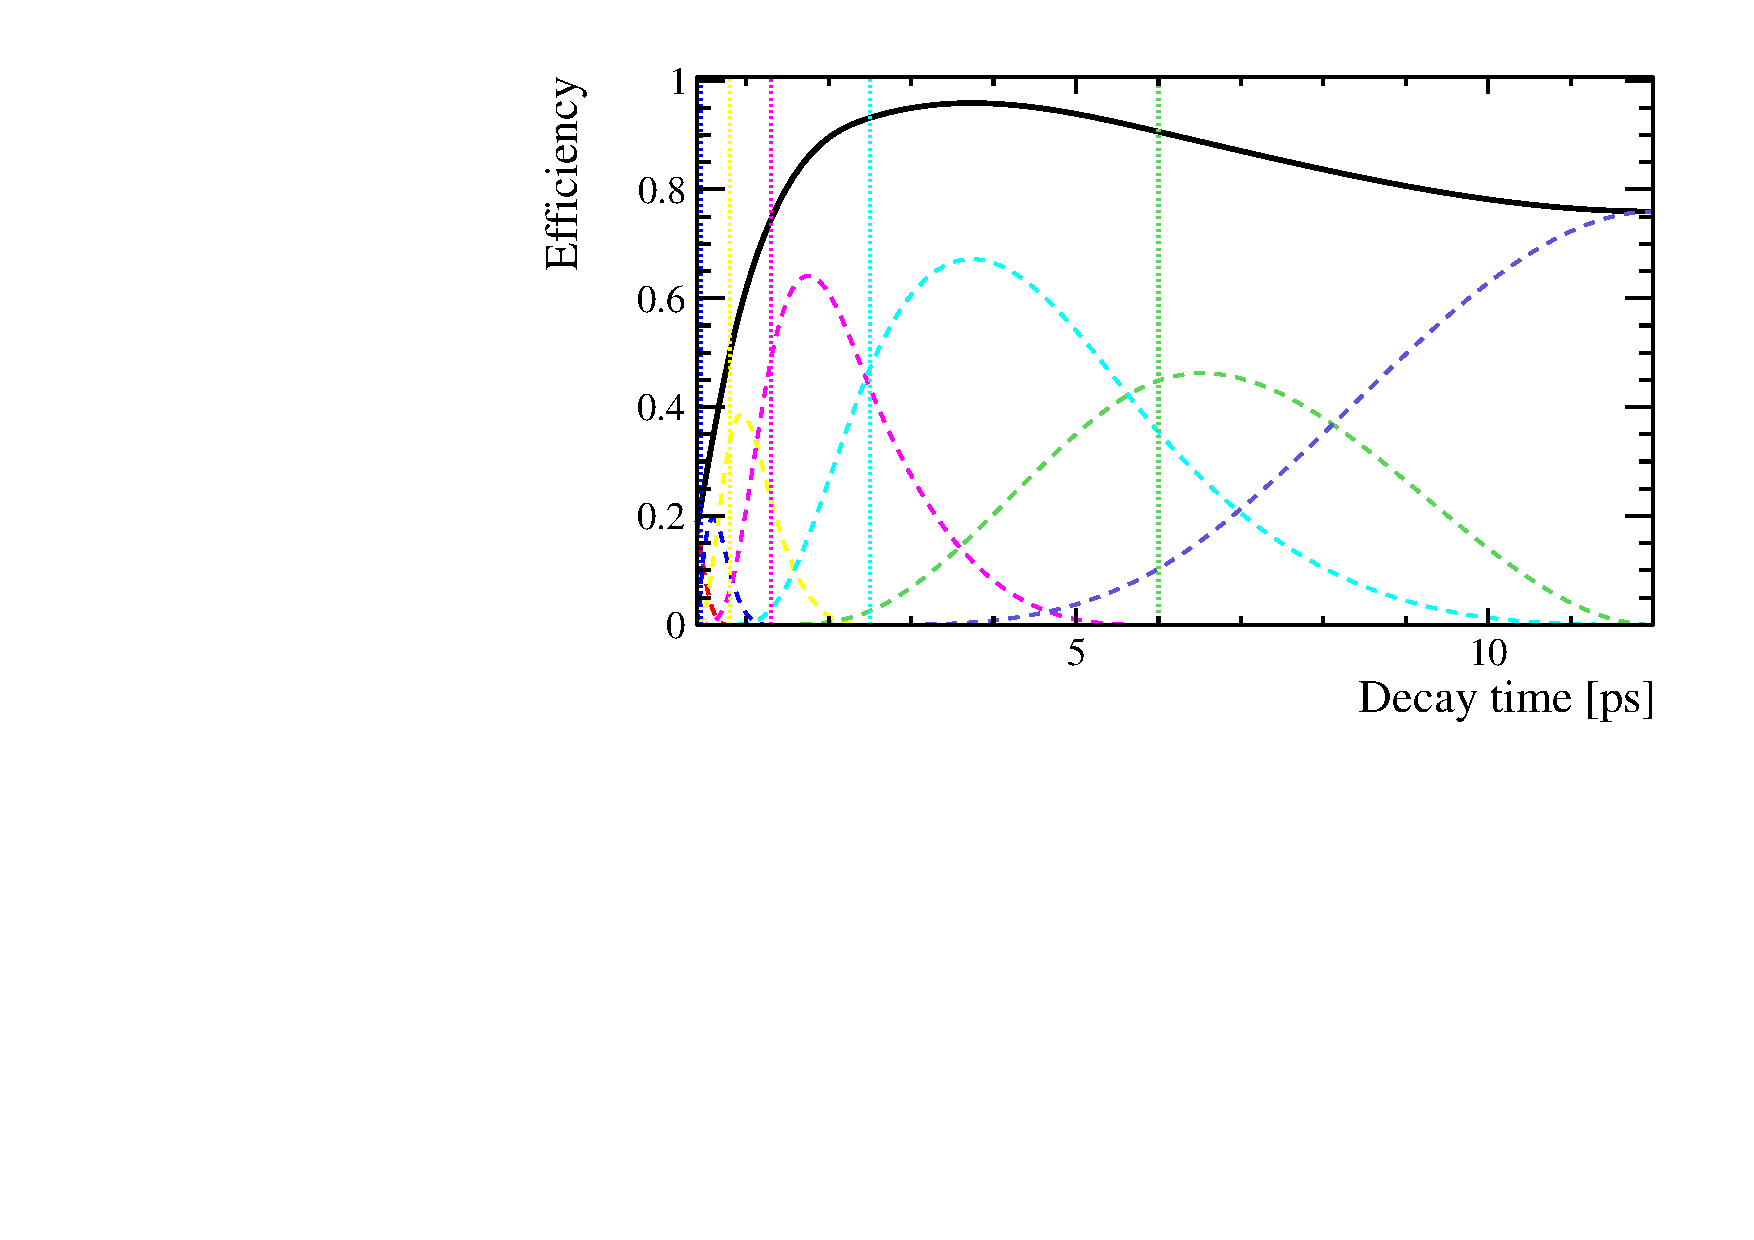
\includegraphics[width=0.8\textwidth]{09TimeFit/figs/Acceptance.pdf}
    \caption{Graphical representation of the acceptance for \BdToDpi.
    The dotted vertical lines represent the knot positions, the dashed lines show the underlying cubic polynomials, where the same colour is chosen for the associated knot and polynomial.}
    \label{fig:acceptance}
\end{figure}

\subsection[head={Extraction of \CP observables},tocentry={Extraction of \CP observables}]{Extraction of $\symbfsf{\CP}$ observables}
\label{sec:ExtractCPobs}

The \CP parameters \Sf and \Sfbar are determined through a multidimensional unbinned maximum-likelihood fit to the by \emph{sWeights} background-subtracted distributions of \BdToDpi.
The PDF to describe the decay time $t$, the tags $\vec{d}=(d^{\text{\tiny OS}}, d^{\text{\tiny SS}})$ and final state $F$ taking the values \f and \fbar, given the mistags $\vec{\eta}=(\eta^{\text{\tiny OS}}, \eta^{\text{\tiny SS}})$ is given by
\begin{equation}
\mathcal{P}(t, F, \vec{d}|\vec{\eta})\propto a(t)\left(P(t', F, \vec{d}|\vec{\eta})\otimes R(t'-t)\right)
\end{equation}
where $P(t', F, \vec{d}|\vec{\eta})$ describes the true decay time, $R(t'-t)$ is the resolution from \cref{sec:resolution} and $a(t)$ parametrises the acceptance described in \cref{sec:acceptance}.
Furthermore the function $P(t', F, \vec{d}|\vec{\eta})$ corresponds to the decay rates from \crefrange{eq:DecRateB2Dmpip}{eq:DecRateBb2Dppim} taking into account the corrections from \cref{eq:decRateCorrectFT}.
Besides, production and detection asymmetry must be described.
These are defined as
\begin{equation}
A_{\text{P}}=\frac{\sigma(\Bzb)-\sigma(\Bz)}{\sigma(\Bzb)+\sigma(\Bz)}\hspace{0.5cm}\text{and}\hspace{0.5cm}A_{\text{D}}=\frac{\varepsilon(\,\f)-\varepsilon(\,\fbar)}{\varepsilon(\,\f)+\varepsilon(\,\fbar)}
\end{equation}
where $\varepsilon$ is the decay-time integrated reconstruction and selection efficiency for the finalstates states \f and \fbar and $\sigma$ is the production cross-section for \Bz and \Bzb mesons.
Both asymmetries were determined to be at the percent level in independent measurements at \lhc energies.
As both are further known to be decay-time independent they can be described by modifying the expressions for the \CP coefficients from \cref{eq:decRateCorrectFT} further to
\begin{equation}
\begin{aligned}
\left(\Delta^--\Delta^+\right)\Sf&\to\left(\Delta^--A_{\text{P}}\,\Delta^+\right)(1+A_{\text{D}})\Sf\\
\left(\Delta^--\Delta^+\right)\Cf&\to\left(\Delta^--A_{\text{P}}\,\Delta^+\right)(1+A_{\text{D}})\Cf.
\end{aligned}
\end{equation}
The same expressions also apply to \Sfbar and \Cfbar with the substitution $A_{\text{D}}\to -A_{\text{D}}$.

As explained in \cref{sec:taggingstrategy}, due to the expected small value of $r$ (see cref{sec:GammaInBd2Dpi}), the parameters \Cf and \Cfbar are fixed to \num{1} and \num{-1}.
Moreover, since possible tagging efficiency asymmetries are measured in simulation to be compatible with zero, they are fixed to this value for the OS and SS taggers.
Possible systematic effects due to one of both assumptions are taken into account in the systematic uncertainties.
Furthermore, the following parameters are constrained by means of a Gaussian function:
\begin{equation}
\begin{aligned}
\tau&=\SI{1.518\pm0.004}{\pico\second}\\
\dm&=\SI{0.5050\pm0.0023}{\per\pico\second}
\end{aligned}
\end{equation}
where for the lifetime $\tau$ the world average~\cite{PDG_2017} is taken and for the oscillation frequency \dm the result of the semi-leptonic \lhcb measurement~\cite{Aaij:2016fdk} is used.
Hence, the free parameters in the fit are the \CP parameters \Sf and \Sfbar, the production and detection asymmetry, the calibration parameters of the OS and SS taggers and the acceptance parameters.
The results of the fits are shown in \cref{tab:DecTimeProjection}, \cref{fig:DecTimeProjection} shows the projection of the PDF onto the decay-time distribution.
\begin{figure}[tbp]
    \centering
    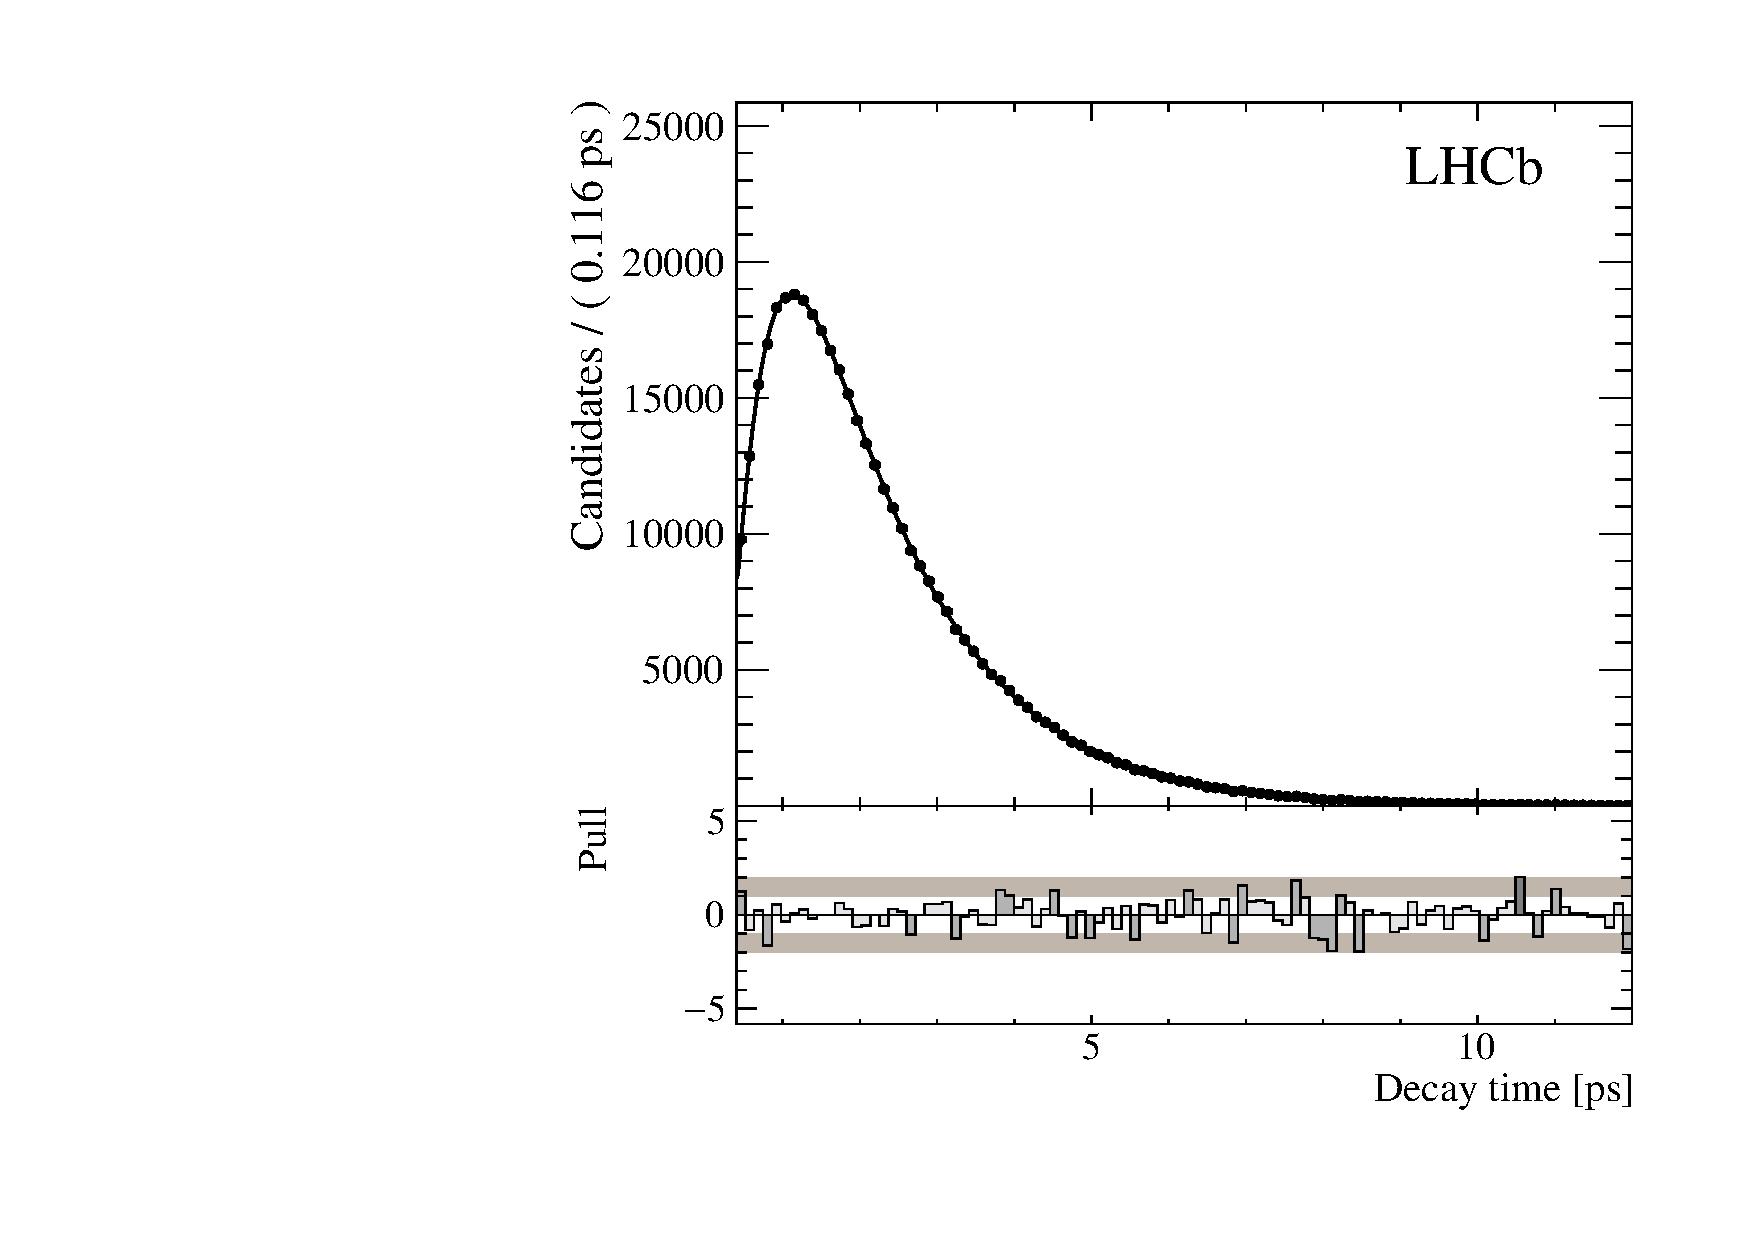
\includegraphics[width=0.7\textwidth]{09TimeFit/figs/BeautyTime_pull.pdf}
    \caption{Background-subtracted decay-time distribution of \BdToDpi candidates.
    The solid curve is the projection of the PDF, the black points represent the data.}
    \label{fig:DecTimeProjection}
\end{figure}

\begin{table}[tbp]
	\centering
	\caption{OS calibration parameters obtained on the $\Bu\!\to\Dz\pip$ data sample.}
	\begin{tabular}{ccccc}
		\toprule
		$p_0$ & $p_1$ & $p_2$ & $p_3$ & $p_4$ \\
		\midrule
		\num{-0.136\pm0.019}  & \num{-0.006\pm0.022} & \num{-0.0107\pm0.0083} &\num{-0.45\pm0.10} &\num{-0.85\pm0.46}\\
		\midrule
		$\Delta p_0$ & $\Delta p_1$ & $\Delta p_2$ & $\Delta p_3$ & $\Delta p_4$ \\
		\midrule
		\num{-0.129\pm0.038}  & \num{0.042\pm0.045} & \num{-0.020\pm0.017} &\num{0.42\pm0.21} &\num{1.91\pm0.92}\\
		\bottomrule
	\end{tabular}
	\label{tab:DecTimeProjection}
\end{table}


\section{Fit validation}
\label{sec:decTimeFitVal}


\subsection{Decay-time fits in subsamples}


\subsection{Decay-time fits to simulated events}
